
\documentclass[journal]{IEEEtran}

\usepackage{color}
\usepackage{isotope}
\usepackage{graphicx,subfigure}
\usepackage{dcolumn}% Align table columns on decimal point
\usepackage{bm}% bold math
\usepackage[utf8]{inputenc}

\usepackage[pdfborder=000,pdftex=true]{hyperref}
\usepackage{amsmath}
\usepackage{balance}

\begin{document}

\title{Software system for data acquisition and real-time analysis operating the ATLAS-TPX Network}

\author{Benedikt~Bergmann, Jakub~Begera, Petr~Burian, Josef~Janecek, Petr~Manek, Stepan~Polansky, Stanislav~Pospisil~\IEEEmembership{Senior~Member,~IEEE}

\thanks{B. Bergmann, J. Begera, P. Burian, J. Janecek, P. Manek, S. Polansky, S. Pospisil are with the Institute of Experimental and Applied Physics, Czech Technical University in Prague, Horska 3a/22, 128 00 Praha 2-Albertov, Czech Republic.

P. Burian is also with the Faculty of Electrical Engineering, University of West Bohemia.\protect\\
The work has been done in the frame of the Medipix collaboration. This research project has been supported by the Ministry of Education, Youth and Sports of the Czech Republic under project numbers: LM2015058 and LG15052\protect\\
E-mail: jakub.begera@cvut.cz, petr.manek@cvut.cz}
}

\markboth{}%
{J. Begera, P. Manek \MakeLowercase{\textit{et al.}}: The ATLAS-TPX detector network}


\maketitle

%\tableofcontents

\begin{abstract}
A network of 15 Timepix pixel detectors was installed within the ATLAS experiment at CERN, Geneva. The network is capable of real-time measurement of the composition and spectral characteristics of the radiation fields. Its operation is managed by a dedicated software system. The presented article describes primary components of this system responsible for communication with detector hardware, online operation monitoring, remote acquisition control, automated data verification and analysis. The processed data can be accessed through an interactive web-based Data Visualization Application, which is publicly available to the scientific community.
\end{abstract}

\section{\label{sec:introduction}Introduction}
The ATLAS-MPX Network has been installed in the ATLAS cavern at the LHC at CERN~\cite{CampbellATLAS}. During the 2013-2014 shut-down period this network was upgraded to a two-layer Timepix design (ATLAS-TPX) with a faster readout system and improved capabilities to discriminate charged particles and gamma rays against neutrons.

Operation of the network is managed by a distributed software system comprised of several independent components:
~
\begin{itemize}
\item The Acquisition and Control Subsystem handles communication with detectors through the readout interface.
\item The Data Analysis Subsystem automatically verifies and processes frames taken by detectors.
\item The Data Visualization Application displays processed data in the form of pixel matrices and trace flux charts.
\end{itemize}

\section{\label{sec:device}Device Design}
Each ATLAS-TPX device consists of two Timepix~\cite{Llopart2007} readout chips with silicon sensor layers of thicknesses 300\,$\mu$m and 500\,$\mu$m facing each other. They are interlaced by a set of neutron converters. The Timepix ASIC (application specific integrated circuit) divides the sensor area into a square matrix of $256 \times 256$ contiguous pixels with a pixel dimension of 55\,$\mu$m. It allows a configuration of each pixel in either of the three modes of operation: 
~
\begin{itemize}
\item In the spectroscopic Time-over-Threshold (ToT) mode the energy deposition in the sensor material is measured.
\item In the Time-of-Arrival (ToA) mode the time from an interaction with respect to the end of the exposure is recorded (precision up to 25\,ns).
\item In the counting mode, the number of interactions with energies above 5\,keV during the exposure time are counted.
\end{itemize}

Data are taken in so-called frames, representing the counter contents of all individual pixels after an adjustable exposure time (often also referred to as frame acquisition time). In each frame, interacting quanta of ionizing radiation can be seen as tracks on the pixel matrix, which have characteristic shapes, depending on the particle range in silicon, its deposited energy, angle of incidence, and particle type. 

\section{\label{sec:hardware}Hardware Architecture}
Given the harsh radiation environment within the ATLAS machine, ATLAS-TPX devices have to be connected to the rest of the system through a dedicated read-out interface. This interface is a special hardware device that reads data and controls acquisition of the detector~\cite{Pixelman}. The ATLASPIX interface (see Fig.~\ref{fig:device_with_readout}) was developed by modifying a regular FITPix interface~\cite{FITPix}.

\begin{figure}[tbp]
	\centering
        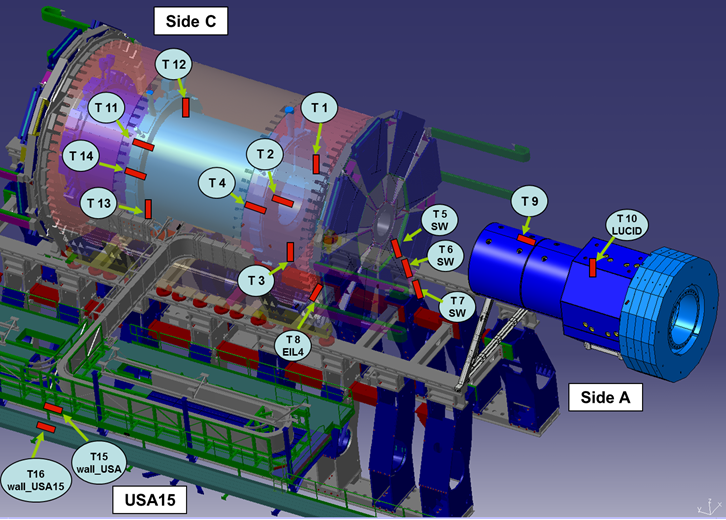
\includegraphics[clip, width=.45\textwidth, angle = 0 ]{Plots/ATLASTPX.png}
      \caption {Artistic view of the device positions of the ATLAS-TPX network in the ATLAS experiment.}
    \label{fig:positions}
\end{figure}

The interface has two parts connected by four cables. The detector itself is positioned and oriented within the ATLAS machine (see Fig.~\ref{fig:positions}), whereas the rest of the interface is placed in a nearby server room, shielded against ionizing radiation. Cables connect both parts, allowing protected hardware to control detectors remotely during operation of the machine. To manage multiple detectors simultaneously, a computer is directly connected to all read-out interfaces. This computer, also known as \textit{the Control PC}, gathers all measured data and forwards commands from the system operator to the detectors through the ATLASPIX interface.

\begin{figure}[tbp]
	\centering
        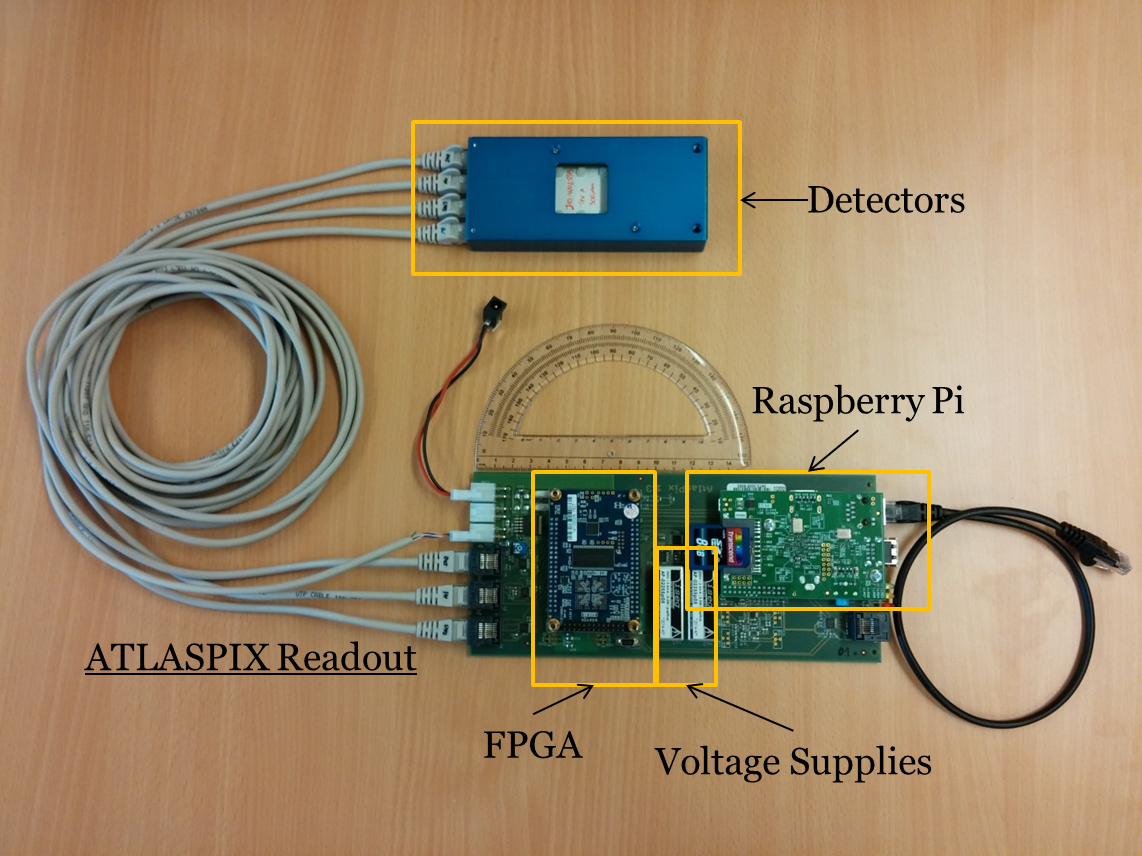
\includegraphics[clip,width=.45\textwidth, angle = 0 ]{Plots/ATLASPIX.png}
      \caption {ATLAS-TPX device, connected to its readout system through three Ethernet cables. The readout system consists of an FPGA, handling the device settings and operation, and a Raspberry Pi minicomputer for sending the data to the control PC in human readable format. Two voltage supplies are used for feeding the proper bias to each of the sensor layers.}
    \label{fig:device_with_readout}
\end{figure}

The Control PC is connected directly to the ATLAS Network, which is isolated from the rest of CERN network infrastructure. Consequently, all communications outside the network have to utilize other systems. Acquisition control and real-time status monitoring of the network uses DCS (Detector Control System). Taken data is transferred to the EOS storage system. Communication between components of the system is depicted in Fig.~\ref{fig:data_flow}.

\begin{figure}[tbp]
	\centering
        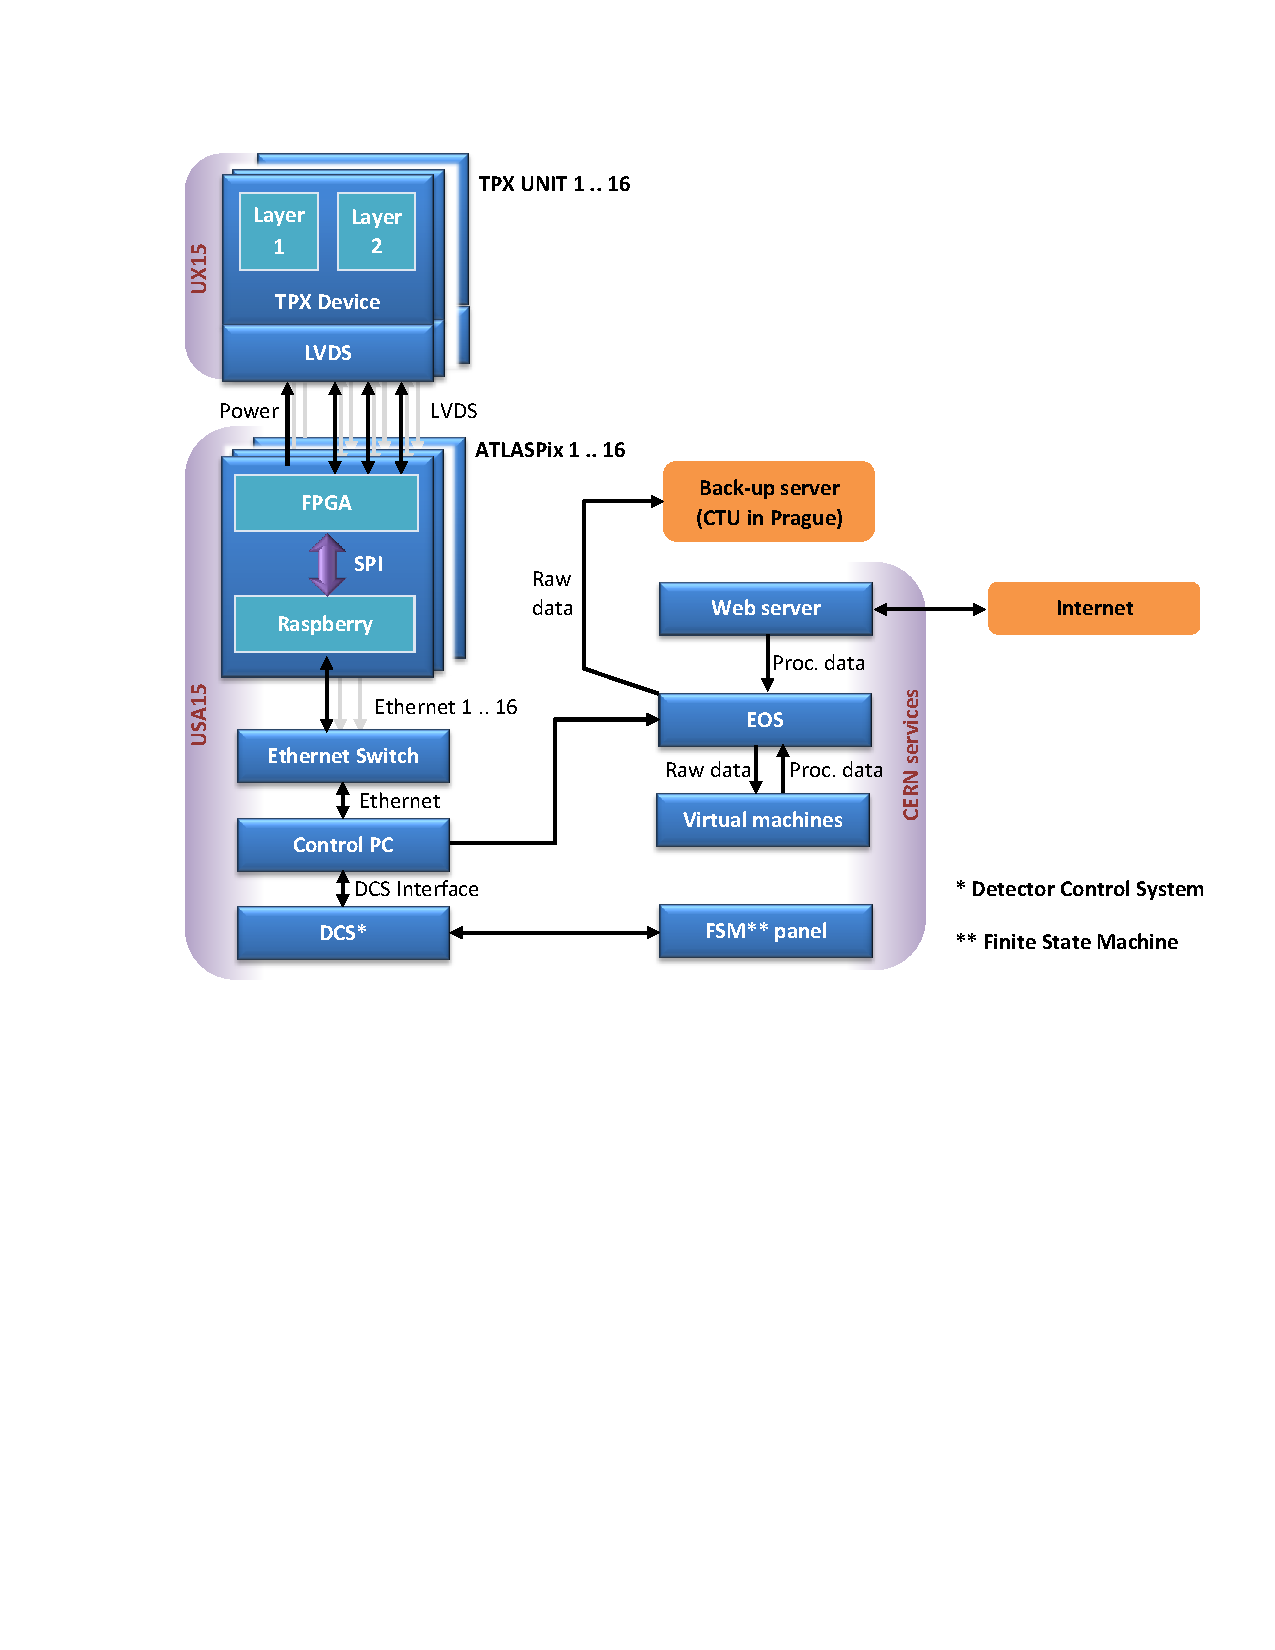
\includegraphics[clip, trim={2cm 11.2cm 0cm 2.6cm}, width=.5\textwidth, angle = 0 ]{Plots/Doc1.pdf}
      \caption {Scheme of the readout, detector control, and data flow.}
    \label{fig:data_flow}
\end{figure}

\section{\label{sec:acquisition}Acquisition \& Control Software}
TODO Jakub

\section{\label{sec:analysis}Data Analysis Subsystem}
The Data Analysis Subsystem is comprised of virtual machines hosted at CERN Meyrin data center and managed by OpenStack private cloud. Each machine provides multitude of \textit{worker nodes} responsible for parallel execution of queued \textit{jobs} -- mutually independent operations that interact with data files. Scheduling and completion of such jobs as well as the heartbeat and load of workers is continuously tracked by a single centralized \textit{manager node}, which indirectly communicates with all workers through shared PostgreSQL database cluster.

The primary purpose of the subsystem is to provide reliable infrastructure for automated data evaluation. For reasons of stability, this task is performed asynchronously with respect to all incoming data. In addition to processing new frames, this approach allows data files to be reprocessed when novel analysis algorithms are introduced.

Frames taken by TPX detectors are temporarily retained at the Control PC, then transferred to the EOS shared disk pool storage in 1-hour batches. Once in EOS, data files become available to all users of the system. Even though subsequent analysis can be performed atop the original data files, their storage format contains reduntant information and is thus not optimal for long-running analysis tasks. For this reason, original data files are first processed and converted into better suited storage format.

The conversion process is automatically scheduled as a job by the manager after the data is confirmed to be valid and no detector malfunctions are suspected. In the course of this operation, frames are subject to cluster analysis \cite{Holy2008} and measurements are combined with energy calibration data. \cite{Jakubek2011} Outputs are stored back in EOS in format compatible with the ROOT Data Analysis Framework. \cite{ROOT}

The produced files serve as a database of the Data Visualization Application. In addition, these files serve as a starting point for other analysis tasks such as activation analysis, noisy pixel detection or luminosity monitoring. The original data files are compressed and downloaded to a backup medium for archivation.

\section{\label{sec:dal}Visualization Application}
Processed data can be examined directly from the ROOT files or by means of the Data Visualization Application. \cite{Manek2016} This application features a simple web interface capable of displaying frames given specific detector, date and time. In addition, the application is capable of plotting fluxes of characteristic traces in specified time periods. See Fig. \ref{fig:positions}.

Since the data is visualized on client-side using modern rendering techniques, the application can also offer basic data operations such as cluster filtering, pixel masking, data aggregation, integral view and logarithmic scale.

The application serves mainly as a tool of manual inspection of the network operation history. It is openly available to the scientific community upon request.

\begin{figure}[tbp]
	\centering
        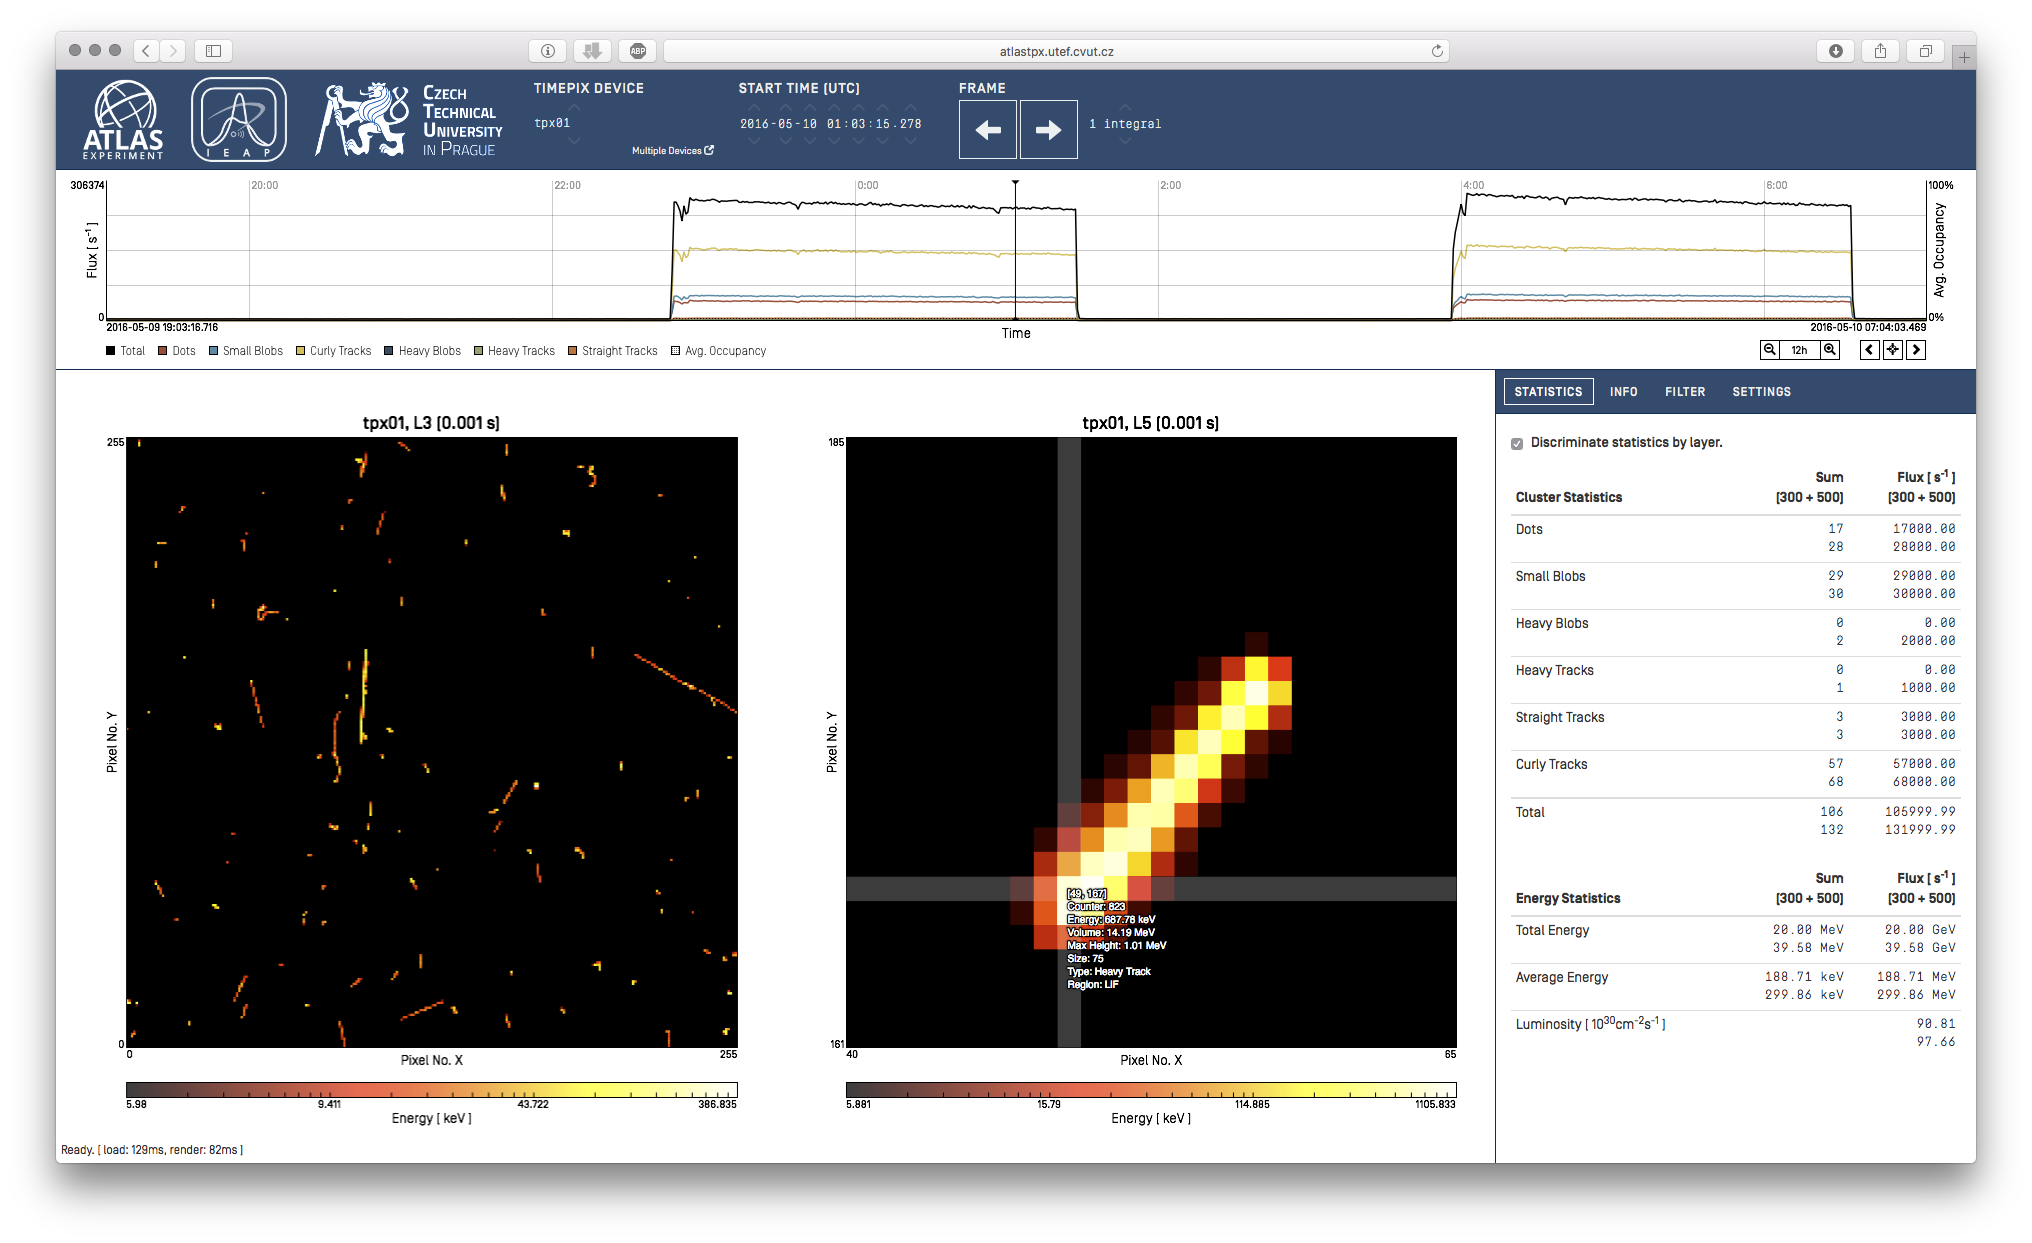
\includegraphics[clip, width=.45\textwidth, angle = 0 ]{Plots/screen-tpx01-crosshair-zoomed.png}
	  \caption {Screenshot of the Data Visualization Application. \cite{Manek2016} Top chart shows flux of characteristic traces in frames in specified time range, bottom charts show pixel matrices at a specified time.}
    \label{fig:positions}
\end{figure}

\section{\label{sec:conclusion}Conclusion}
The presented software can successfully control detector acquisition and retrieve, analyze and display frames from the ATLAS-TPX network. All components of the system are fully operational. The Data Visualization Application is publicly available to the scientific community upon request.


%
\bibliographystyle{IEEEtran}
\bibliography{ieee2016}% Produces the bibliography via BibTeX.
%\begin{thebibliography}{10}
%\end{thebibliography}
%
\end{document}
%
% ****** End of file apssamp.tex ******
